\section{Convergencia}
\label{section:convergence}

Las simulaciones se realizaron empleando el software \textit{Computer Simulation Technology} (CST, versión 2025) en una computadora de escritorio equipada con un procesador Intel Core i7 de $13^a$ generación (16 núcleos, 24 hilos) y 64 GB de memoria RAM, bajo el sistema operativo Windows. El análisis de convergencia se llevó a cabo mediante la comparación entre la solución analítica para una esfera, descrita por la teoría de Mie \cite{bohrenAbsorptionScatteringLight2008}, y los resultados numéricos obtenidos con CST. Para este propósito, se consideró una esfera de radio 2,680 nm, cuya función dieléctrica corresponde a la de un eritrocito con una CHCM de 30.6 g/dL, inmersa en plasma con $\varepsilon_{\text{Plasma}}=~1.823$. La esfera se iluminó con una onda plana propagándose en la dirección $z$ y polarizada en $x$, considerando longitudes de onda el rango de 400 a 600 nm. En CST se evaluó la influencia de distintos parámetros numéricos sobre la convergencia de la solución, entre ellos: el tamaño del dominio computacional --definido por la distancia entre la partícula y la caja de simulación (\textit{bounding box})--, el nivel de reflexión estimado (\textit{estimated reflection level}) --relacionado con la capa absorbente Perfect Matching Layer (PML)--, así como el mallado global y el mallado local (tanto en volumen como en superficie). A lo largo del análisis, estos parámetros se ajustaron con el fin de minimizar las discrepancias numéricas respecto a la solución analítica de Mie y garantizar la convergencia de las simulaciones. En la Fig.~\ref{subfig:CST_matriz} se muestra la geometría del problema, donde la esfera se encuentra inmersa en el dominio delimitado por la caja de simulación. Por otro lado, en la Fig.~\ref{subfig:CST_mesh} se muestran algunos de los parámetros de discretización considerados. El mallado global corresponde a la discretización de todo el dominio (matriz y partícula), mientras que, en caso de emplearse un refinamiento local, este se aplica exclusivamente a la partícula. Asimismo, se define la distancia $h$ como la separación mínima entre la superficie de la partícula y la caja de simulación. 

\begin{figure}[h]
	\centering
	\sidesubfloat[First image]{{
			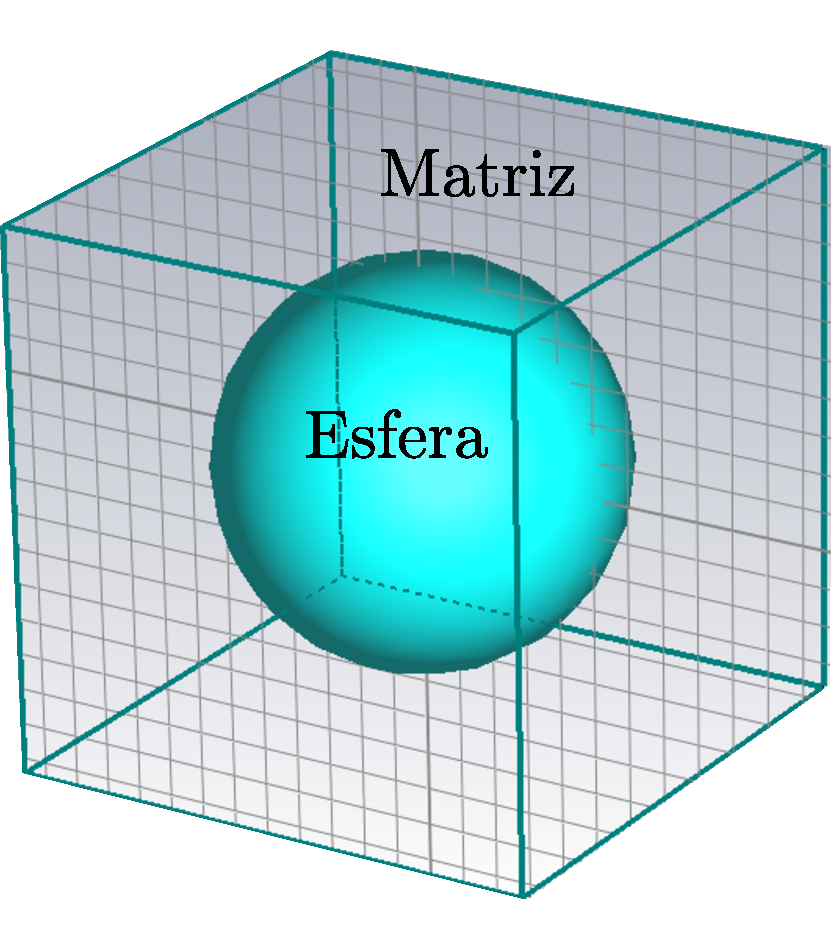
\includegraphics[width=5cm]{../../Figuras/3-FIT/Matriz.pdf}\label{subfig:CST_matriz}}}\hspace{0.1cm}
	\sidesubfloat[Second image]{{	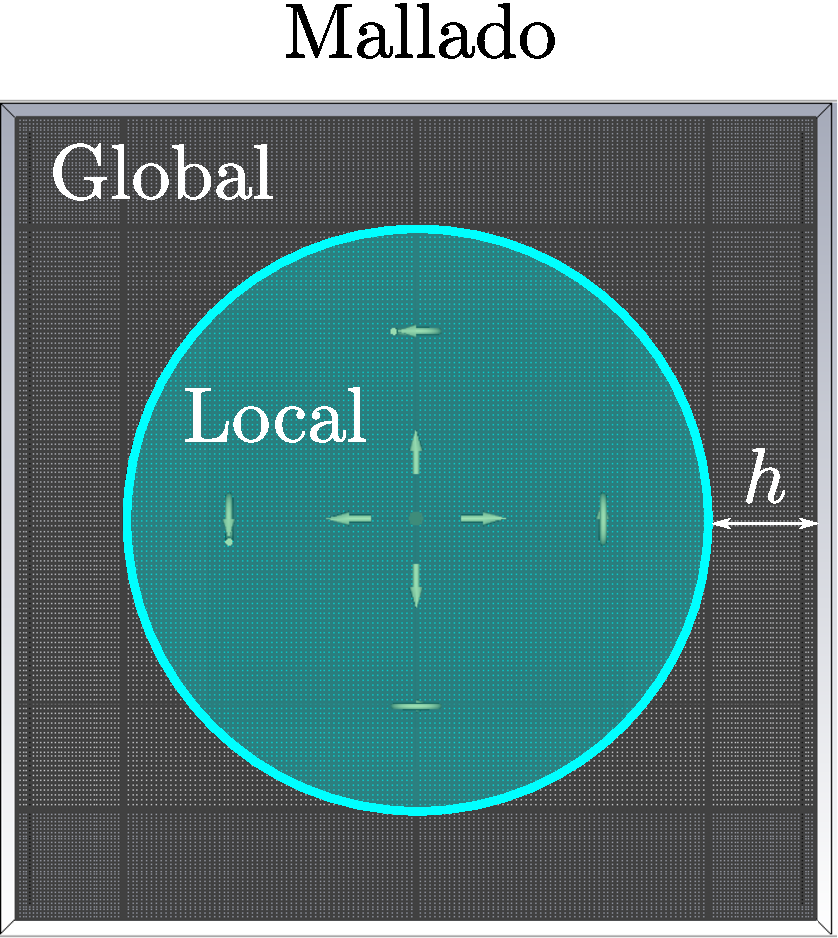
\includegraphics[width=4.55cm]{../../Figuras/3-FIT/Mesh.pdf}\label{subfig:CST_mesh}}}\vspace{-0.1cm}
	\caption{\textbf{a)} Vista tridimensional del dominio computacional en CST.  \textbf{b)} Corte transversal del mallado del dominio computacional en CST. Se indica el mallado global como todo lo que rodea a la esfera, el mallado local como lo que compone a la esfera y la distancia $h$ entre el borde de la esfera y el borde de la caja de simulación.}
	\label{fig:CST}
\end{figure}
%

Para evaluar la influencia de la distancia $h$ en $Q_{\text{ext}}$ y su diferencia con respecto a la solución analítica de teoría de Mie para una esfera de radio 2,680 nm, con función dieléctrica corresponde de un eritrocito con una CHCM de 30.6 g/dL, inmersa en plasma con $\varepsilon_{\text{Plasma}}=~1.823$, se emplearon los parámetros predeterminados de CST: un mallado global definido por 15 celdas por longitud de onda, sin refinamiento local, y un nivel de reflexión de $10^{-5}$ (cercano al valor recomendado de $10^{-4}$). En la Fig.~\ref{fig:ajusteMatriz} se muestra $Q_{\text{ext}}$ en función de la longitud de onda incidente $\lambda$ para distintos valores de $h$: 500, 1000, 1230, 1470, 1720 y 2300 nm que se identificaron mediante puntos de color negro, morado, vino, naranja oscuro, naranja claro y amarillo, respectivamente. La línea continua que une los puntos es una guía visual. Asimismo, se muestra la solución analítica obtenida mediante teoría de Mie como una línea continua verde. En la solución analítica se observan tres mínimos espectrales asociados a los centros de las principales bandas de absorción descritas por la función dieléctrica: la banda de Soret, centrada alrededor de 428 nm, y las bandas $\beta$ y $\alpha$, centradas aproximadamente en 541 nm y 575 nm, respectivamente. El espectro completo de 400 a 600 nm se presenta en la Fig.~\ref{subfig:ajusteMatrizGlobal}, mientras que en las Figs.~\ref{subfig:ajusteMatrizSoret}, \ref{subfig:ajusteMatrizBeta} y \ref{subfig:ajusteMatrizAlpha} se muestran ampliaciones en las regiones correspondientes a la banda de Soret y a las bandas $\beta$ y $\alpha$. 
%
\begin{figure}[h!]
	\centering
	\sidesubfloat[First image]{\hspace{-0.1cm}{
			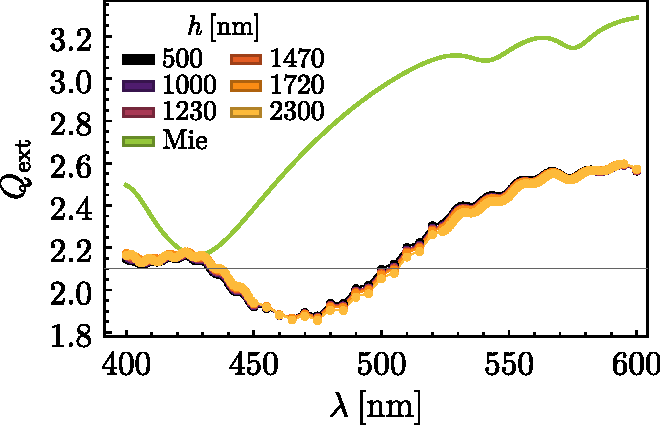
\includegraphics[width=0.45\textwidth]{../Figuras/3-FIT/ajusteMatriz.pdf}\label{subfig:ajusteMatrizGlobal}}}\hspace{0.1cm}
	\sidesubfloat[Second image]{\hspace{-0.1cm}{	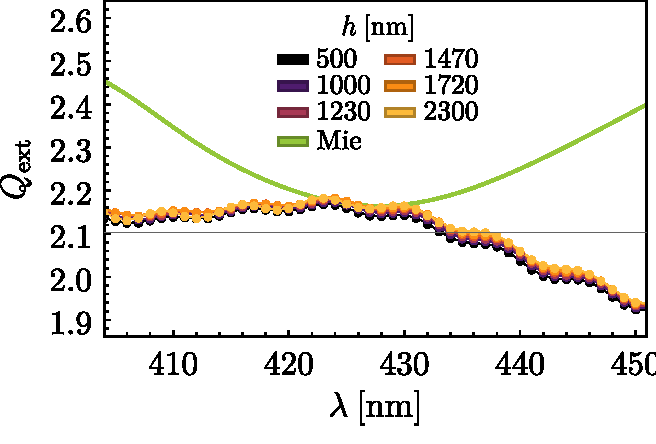
\includegraphics[width=0.45\textwidth]{../Figuras/3-FIT/ajusteMatrizSoret.pdf}\label{subfig:ajusteMatrizSoret}}}
	
	\vspace{0.3cm}
	
	\sidesubfloat[Third image]{\hspace{-0.1cm}{	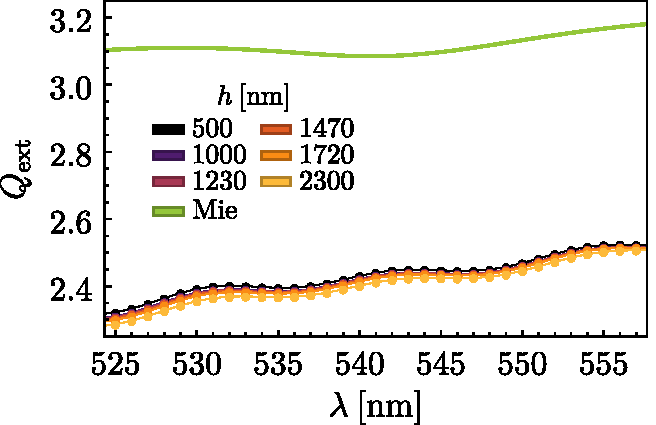
\includegraphics[width=0.45\textwidth]{../Figuras/3-FIT/ajusteMatrizBeta.pdf}\label{subfig:ajusteMatrizBeta}}}	\hspace{0.1cm}
	\sidesubfloat[Fourth image]{\hspace{-0.1cm}{	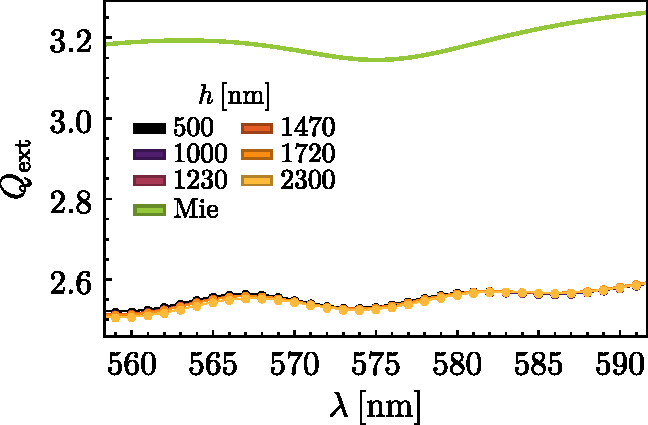
\includegraphics[width=0.45\textwidth]{../Figuras/3-FIT/ajusteMatrizAlpha.pdf}\label{subfig:ajusteMatrizAlpha}}}
	
	
	\caption{Eficiencias de extinción $Q_{\text{ext}}$ para una esfera de radio de 2,680 nm con función dieléctrica correspondiente a un eritrocito con CHCM de 30.6 g/dL iluminada con una onda plana en función de la longitud de onda $\lambda$. Se comparan los datos obtenidos mediante CST con  valores de $h$ de 500, 1000, 1230, 1570, 1720 y 2300 nm que se identifican mediante puntos de color negro, morado, vino, naranja oscuro, marajna claro y amarillo, respectivamente. La línea continua que une los puntos es una guía visual. Se incluye también la solución analitíca de teoría de Mie (línea verde continutua)  \textbf{a)} Espectro de 400 a 600 nm. \textbf{b)} Región asociada a la banda de Soret \textbf{c)} Región asociada a la banda $\beta$. \textbf{d)} Región asociada a la banda $\alpha$.  }
	\label{fig:ajusteMatriz}
\end{figure}
%

A partir de estos resultados, se observa un desfase en el mínimo global entre la solución numérica y la analítica, así como la presencia de oscilaciones en todo el espectro. Dado que estas oscilaciones no se observan en la solución analítica, se espera que no correspondan a un comportamiento físico del sistema. Asimismo, se observa una mayor frecuencia de oscilación a menores longitudes de onda por ejemplo, en la región de la banda de Soret las oscilaciones tienen un \textit{Full Width Half Maximum} (FWHM) de 8 nm, mientras que en la región de las bandas $\alpha$ y $\beta$ de aproximadamente 11 nm y 10 nm, respectivamente. En cuanto a la influencia de la distancia $h$, se observa que en la región de la banda de Soret el error\footnote{Se considera al error absoluto a una longitud de onda dada como
	$$\text{Error}(\lambda)=|Q_{\text{CST}}(\lambda)-Q_{\text{Mie}}(\lambda)|,$$
	mientras que el error absoluto promedio se consudera como 
$$\text{Error promedio}=\frac{1}{N}\Sum_i|Q_{\text{CST}}(\lambda_i)-Q_{\text{Mie}}(\lambda_i)|,$$
donde $N$ es el número total de datos promediados.} entre la solución de Mie con la solución analítica disminuye al incrementar $h$ alcanzando valores de hasta 0.022. En contraste, en las bandas $\alpha$ y $\beta$ el error aumenta para valores menores de $h$ alcanzando valores de 0.64. Considerando el comportamiento global en todo el rango espectral, así como el costo computacional asociado (82 minutos), se seleccionó $h$=1000~nm como un valor conveniente para las simulaciones posteriores, dado que el ajuste de otros parámetros podría incrementar significativamente el tiempo de cómputo.


El análisis de la influencia del mallado global se realizó mediante la variación del número de celdas por longitud de onda. Para este estudio no se consideró refinamiento local y se fijó el nivel de reflexión en $10^{-5}$. En la Fig.~\ref{fig:ajusteMesh} se muestra la $Q_{\text{ext}}$ en función de la longitud de onda de la luz incidente, comparando los resultados obtenidos mediante CST con la solución analítica de Mie. El espectro completo se presenta en la Fig. \ref{subfig:ajusteMeshGlobal}, mientras que en las Figs. \ref{subfig:ajusteMeshBeta} y \ref{subfig:ajusteMeshAlpha} se muestran ampliaciones en las regiones correspondientes a la banda de Soret y a las bandas $\beta$ y $\alpha$. El número de celdas por longitud de onda determina directamente el tamaño mínimo de celda en la discretización. En este caso, se consideraron valores de 7, 10, 12, 15 y 17 celdas por longitud de onda, correspondientes a tamaños de celda de 40.0, 28.2, 23.5, 18.7 y 16.5 nm, respectivamente. Estos puntos se representan mediante un gradiente de color rosa, que va de tonos más oscuros para los valores menores (7 celdas por longitud de onda) a tonos más claros para los valores mayores (17 celdas por longitud de onda).  También se muestra la solución analítica de Mie como referencia como una línea continua verde. Se observa que en las regiones de la banda de Soret, $\beta$ y $\alpha$ conforme aumenta el tamaño mínimo de celda, las desviaciones respecto a la solución analítica aumentan. Estas discrepancias se manifiestan como oscilaciones espurias y un desplazamiento en la posición del mínimo global, lo que indica que la discretización es insuficiente para describir adecuadamente la respuesta electromagnética de la partícula. A medida que se refina el mallado la discrepancia entre los resultados de CST y la solución de Mie disminuye de forma sistemática. En particular, para el mallado más fino considerado se obtiene el menor error absoluto promedio, igual a 0.49. No obstante, incluso en este caso persiste un desplazamiento del mínimo global de 37 nm. Considerando el compromiso entre precisión y costo computacional, se seleccionó un mallado de 15 celdas por longitud de onda, ya que la mejora obtenida al incrementar a 17 celdas es poco significativa (del orden de $10^{-3}$ en error absoluto promedio), mientras que el tiempo de simulación aumenta 50 minutos adicionales.
%
\begin{figure}[tb]
	\centering	\sidesubfloat[First image]{\hspace{-0.1cm}{
			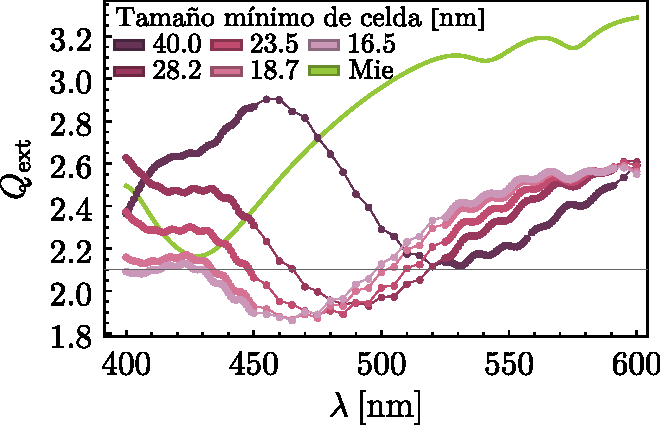
\includegraphics[width=0.45\textwidth]{../Figuras/3-FIT/ajusteMesh.pdf}\label{subfig:ajusteMeshGlobal}}}\hspace{0.1cm}
	\sidesubfloat[Second image]{\hspace{-0.1cm}{	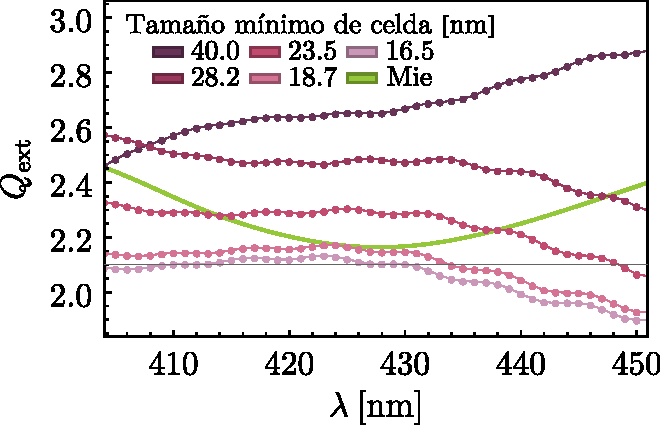
\includegraphics[width=0.45\textwidth]{../Figuras/3-FIT/ajusteMeshSoret.pdf}\label{subfig:ajusteMeshSoret}}}
	
	\vspace{0.3cm}
	
	\sidesubfloat[Third image]{\hspace{-0.1cm}{	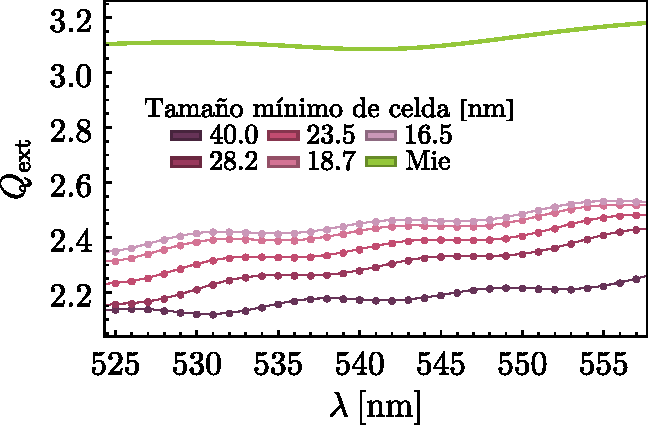
\includegraphics[width=0.45\textwidth]{../Figuras/3-FIT/ajusteMeshBeta.pdf}\label{subfig:ajusteMeshBeta}}}	\hspace{0.1cm}
	\sidesubfloat[Fourth image]{\hspace{-0.1cm}{	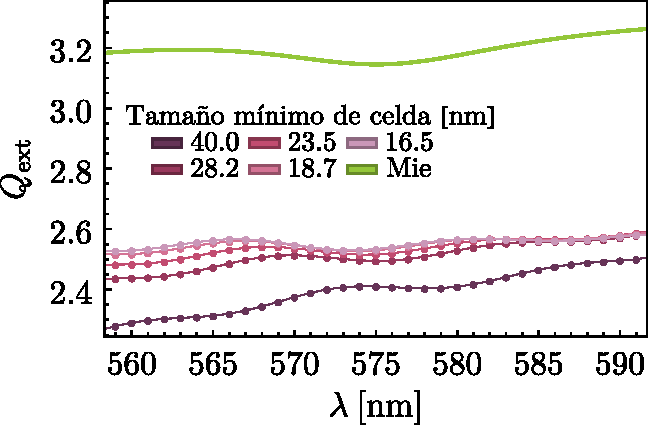
\includegraphics[width=0.45\textwidth]{../Figuras/3-FIT/ajusteMeshAlpha.pdf}\label{subfig:ajusteMeshAlpha}}}
	
	
	\caption{Eficiencias de extinción $Q_{\text{ext}}$ para una esfera de radio de 2680 nm con función dieléctrica correspondiente a un eritrocito con CHCM de 30.6 g/dL iluminada con una onda plana en función de la longitud de onda $\lambda$. Se comparan los datos obtenidos mediante CST con tamaños mínimos de celda iguales a 40, 28.2, 23.5, 18.7 y 16.5 nm que se identifican mediante un gradiente de color rosa que va desde tonos más oscuros a tonos más claros. La línea continua que une los puntos es una guía visual. Se incluye también la solución analitíca de teoría de Mie (línea verde continutua)  \textbf{a)} Espectro de 400 a 600 nm. \textbf{b)} Región asociada a la banda de Soret. \textbf{c)} Región asociada a la banda $\beta$. \textbf{d)} Región asociada a la banda $\alpha$. }
	\label{fig:ajusteMesh}
\end{figure}
%


Con el fin de analizar la influencia del mallado local se evaluó el refinamiento en la superficie y en el volumen de la partícula. Sin embargo, en cuanto al mallado de la superficie no se observaron variaciones ni en $Q_{\text{ext}}$ ni en el tiempo de simulación, por lo que no se incluyen los resultados correspondientes. Este comportamiento puede explicarse por la técnica de \textit{Perfect Boundary Approximation} (PBA) implementada en CST, la cual permite representar con alta precisión superficies curvas sin necesidad de refinamientos adicionales en la discretización geométrica \cite{dassaultsystemesUnderstandingTimeDomain2010}. 

Para evaluar el efecto del mallado local en el volumen de la esfera se fijaron los parámetros previamente optimizados: $h=1000$ nm, un mallado global de 15 celdas por longitud de onda y un nivel de reflexión de $10^{-5}$, variando únicamente el tamaño mínimo absoluto de celda dentro de la partícula. En la Fig.~\ref{fig:ajusteLocalMesh} se muestran los resultados obtenidos de $Q_{\text{ext}}$ para tamaños de celda de 20, 16, 15, 12 y 10 nm, los cuales corresponden a tamaños efectivos mínimos dentro de la esfera de 16.17, 15.95, 14.83, 11.96 y 9.93 nm, respectivamente. Los resultados se representan mediante un gradiente de color morado, que varía desde tonos más oscuros para el mayor tamaño mínimo de celda hasta tonos más claros para el menor. Adicionalmente, se incluye la solución analítica de la teoría de Mie como una línea continua de color verde. El espectro completo se presenta en la Fig. \ref{subfig:ajusteMeshGlobal}, mientras que en las Figs. \ref{subfig:ajusteLocalMeshSoret}, \ref{subfig:ajusteLocalMeshBeta} y \ref{subfig:ajusteLocalMeshAlpha} se muestran ampliaciones en las regiones correspondientes a la banda de Soret y a las bandas Q ($\beta$ y $\alpha$). Se observa que, al disminuir el tamaño de celda, los resultados numéricos convergen progresivamente hacia la solución analítica. Asimismo, la inclusión del mallado local en el volumen de la partícula elimina las oscilaciones espurias observadas previamente, confirmando su origen numérico asociado a una discretización insuficiente de la geometría. Con base en estos resultados, se seleccionó un tamaño mínimo de celda de 10 nm, al representar un equilibrio entre precisión y costo computacional. Cabe señalar que refinamientos adicionales no fueron considerados debido a limitaciones de memoria RAM del equipo de cómputo empleado.
%
\begin{figure}[tb]
	\centering
	\sidesubfloat[First image]{\hspace{-0.1cm}{
			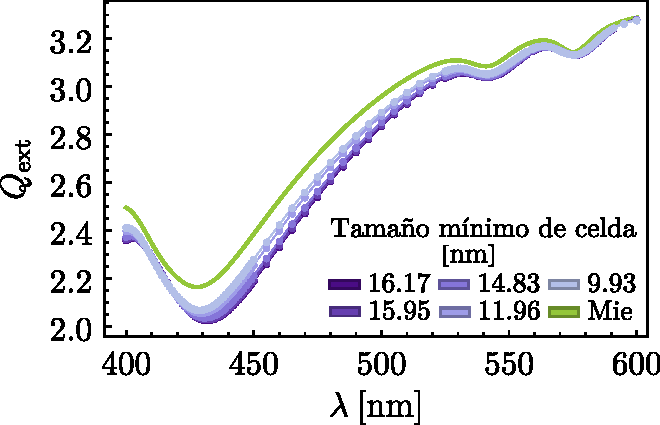
\includegraphics[width=0.45\textwidth]{../Figuras/3-FIT/ajusteMeshLocal.pdf}\label{subfig:ajusteLocalMeshGlobal}}}\hspace{0.1cm}
	\sidesubfloat[Second image]{\hspace{-0.1cm}{	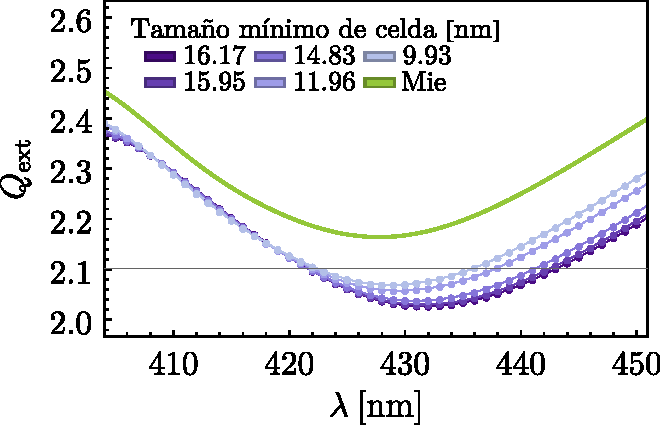
\includegraphics[width=0.45\textwidth]{../Figuras/3-FIT/ajusteMeshLocalSoret.pdf}\label{subfig:ajusteLocalMeshSoret}}}
	
	\vspace{0.3cm}
	
	\sidesubfloat[Third image]{\hspace{-0.1cm}{	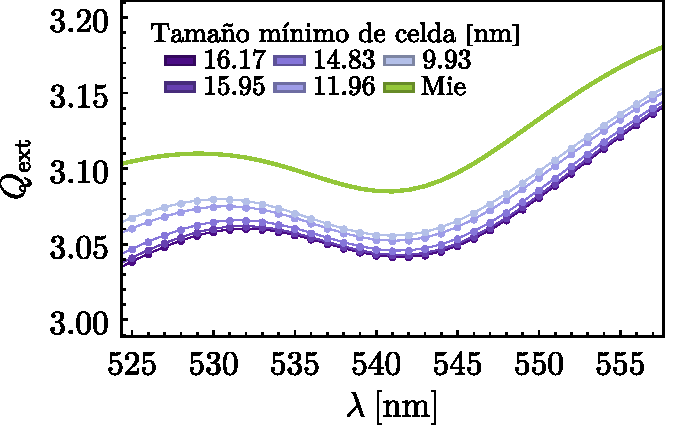
\includegraphics[width=0.45\textwidth]{../Figuras/3-FIT/ajusteMeshLocalBeta.pdf}\label{subfig:ajusteLocalMeshBeta}}}	\hspace{0.1cm}
	\sidesubfloat[Fourth image]{\hspace{-0.1cm}{	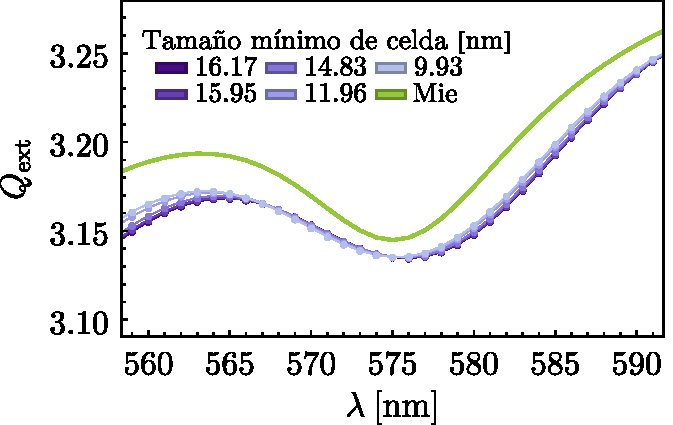
\includegraphics[width=0.45\textwidth]{../Figuras/3-FIT/ajusteMeshLocalAlpha.pdf}\label{subfig:ajusteLocalMeshAlpha}}}
	
	
	\caption{Eficiencias de extinción $Q_{\text{ext}}$ para una esfera de radio de 2680 nm con función dieléctrica correspondiente a un eritrocito con CHCM de 30.6 g/dL iluminada con una onda plana en función de la longitud de onda $\lambda$. Se comparan los datos obtenidos mediante CST con tamaños mínimos de celda iguales a 16.17, 15.95, 14.83, 11.96 y 9.93 nm que se identifican mediante un gradiente de color morado que va desde tonos más oscuros a tonos más claros. La línea continua que une los puntos es una guía visual. Se incluye también la solución analitíca de teoría de Mie (línea verde continua)  \textbf{a)} Espectro de 400 a 600 nm. \textbf{b)} Región asociada a la banda de Soret. \textbf{c)} Región asociada a la banda $\beta$. \textbf{d)} Región asociada a la banda $\alpha$. }
	\label{fig:ajusteLocalMesh}
\end{figure}
%

Empleando los valores previamente optimizados, se analizó la influencia del nivel de reflexión estimado, considerando valores de $ 10^{-4},  10^{-6}, 10^{-8}, 10^{-10}$. No se observan diferencias en los valores de $Q_{\text{ext}}$, sin embargo a medida que disminuye el nivel de reflexión hay incremento en el tiempo de simulación.

 En la Fig.~\ref{fig:tiempos} se muestran los tiempos de simulación (en minutos) en función de las distintas variaciones de parámetros consideradas. Se presentan los resultados conforme se realizó la variación de parámetros, es decir, de izquierda a derecha se muestran los resultados correspondientes a la variación de la distancia $h$, el mallado global, el mallado local en volumen y el nivel de reflexión asociado a la capa absorbente (PML). Cada punto está identificado mediante el mismo código de color empleado en las figuras anteriores, mientras que en color verde se indica el valor seleccionado como óptimo en cada caso. Con base en el análisis conjunto de la convergencia y el costo computacional, los parámetros finales seleccionados son: $h=1000$ nm, mallado global con 15 celdas por longitud de onda, mallado local con un tamaño mínimo de celda de 10 nm y nivel de reflexión estimado de $10^{-4}$. Esta configuración produce un error absoluto promedio de aproximadamente 0.05 respecto a la solución analítica de Mie, con un tiempo total de simulación de alrededor de 770 minutos.
%
\begin{figure}[tb]
	\centering
		\includegraphics[width=1\textwidth]{../Figuras/3-FIT/tiempos_convergencia.pdf}
	
	\caption{Tiempo de ejecución de las simulaciones realizadas en CST. En orden de izquierda a derecha se observa el tiempo de simulación en función de $h$, del tamaño mínimo de celda y del nivel de reflexión para cada uno de los parámetros optimizados: distancia borde-esfera, el mallado global, el mallado local y el PML.
	  }
	\label{fig:tiempos}
\end{figure}
%

Con los parámetros previamente seleccionados, se realizó una verificación adicional de los criterios de convergencia empleados. Para ello, se fijó un tamaño mínimo de celda de 10 nm y se repitió el análisis de la distancia borde-esfera con valores de $h$=950, 1000 y 1050 nm y del mallado global con valores de 12, 15 y 17 celdas por longitud de onda. Los resultados obtenidos se compararon con la solución analítica de Mie en tres longitudes de onda representativas: 428, 529 y 563 nm. Estas longitudes corresponden, respectivamente, al mínimo asociado a la banda de Soret y a los máximos asociados a las bandas $\beta$ y $\alpha$ respectivamente. En la Tabla \ref{table:convergencia} se muestran los valores de $Q_{\text{ext}}$ obtenidos así como el error relativo con respecto a la solución analítica de Mie para distintos valores del mallado global y de $h$. En la tabla de la izquierda se mantiene fijo un mallado global de 15 celdas por longitud de onda mientras se varía $h$. Por su parte, en la tabla de la derecha se fija el valor de $h=1000$ nm y se modifica el número de celdas por longitud de onda.
%
\begin{table}[h!]
	\centering
	
	\begin{tabular}{cc}
		% -------- BLOQUE 1 --------
		\begin{minipage}{0.45\textwidth}
			\centering
			\begin{tabular}{ccc}
				\hline
				\multicolumn{3}{c}{15 celdas por longitud de onda}\\ 
				\hline
				$\lambda$ & $Q_{\text{ext}}$ & Error relativo\\
				\hline
				\multicolumn{3}{c}{$h=950$ nm} \\
				\hline
				428 & 2.07084 & 4.56847 \\
				529 & 3.07943 & 0.994313 \\
				563 & 3.17225 & 0.670544 \\
				\hline
				\multicolumn{3}{c}{$h=1000$ nm} \\
				\hline
				428 & 2.06953 & 4.57459 \\
				529 & 3.07902 & 1.0078 \\
				563 & 3.17233 & 0.668147 \\
				\hline
				\multicolumn{3}{c}{$h=1050$ nm} \\
				\hline
				428 & 2.06824 & 4.64005 \\
				529 & 3.07854 & 1.0235 \\
				563 & 3.17232 & 0.668147 \\
				\hline
			\end{tabular}
		\end{minipage}
		&
		% -------- BLOQUE 2 --------
		\begin{minipage}{0.45\textwidth}
			\centering
		\begin{tabular}{ccc}
			\hline
			\multicolumn{3}{c}{$h=1000$ nm}\\ 
			\hline
			$\lambda$ & $Q_{\text{ext}}$ & Error relativo\\
			\hline
			\multicolumn{3}{c}{12 celdas por longitud de onda} \\
			\hline
			428 & 2.04120 & 6.02605 \\
			529 & 3.06460 & 1.48286 \\
			563 & 3.16445 & 0.918616 \\
			\hline
			\multicolumn{3}{c}{15 celdas por longitud de onda} \\
			\hline
			428 & 2.06953 & 4.57459 \\
			529 & 3.07902 & 1.00780 \\
			563 & 3.17233 & 0.66814 \\
			\hline
			\multicolumn{3}{c}{17 celdas por longitud de onda} \\
			\hline
			428 & 2.07888 & 4.10444 \\
			529 & 3.08384 & 0.84972 \\
			563 & 3.17484 & 0.58853 \\
			\hline
		\end{tabular}
		\end{minipage}
	\end{tabular}
	
	\caption{Valores de $Q_{\text{ext}}$ y errores relativos respecto a la solución analítica de Mie, considerando un refinamiento local con tamaño mínimo de celda de 10 nm. En la tabla izquierda se muestran los resultados obtenidos para un mallado global de 15 celdas por longitud de onda y valores de $h=950, 1000$ y 1500 nm. En la tabla derecha se presentan los resultados para $h=1000$ nm y mallados globales de 12, 15 y 17 celdas por longitud de onda.}
	\label{table:convergencia}
\end{table}
%

Se observa que en la longitud de onda de 428 nm las diferencias aparecen a partir de la segunda o tercera cifra decimal de $Q_{\text{ext}}$, mientras que para 529 y 563 nm las discrepancias se restringen principalmente a la tercera y cuarta cifras decimales. Los errores relativos muestran que las tendencias observadas en los análisis iniciales se conservan tras la incorporación del mallado local. Por otra parte, el mallado de 17 celdas por longitud de onda presenta la mejor concordancia con la solución analítica de Mie en las tres longitudes de onda consideradas, alcanzando errores relativos inferiores al 4.2\%. Asimismo, el incremento en el costo computacional asociado resulta moderado, ya que el tiempo de simulación aumenta únicamente alrededor de 30 minutos respecto al caso de 15 celdas por longitud de onda. Con base en estos resultados, se adoptó finalmente la combinación $h=1000$ nm y un mallado global de 17 celdas por longitud de onda para las simulaciones posteriores.



